% KitchenSnitchserver-DK.tex
\begin{hcarentry}[new]{Kitchen Snitch server}
\report{Dino Morelli}
\status{stable, actively developed}
\participants{Betty Diegel}
\makeheader

This project is the server-side software for Kitchen Snitch, a mobile
application that provides health inspection scores, currently for the
Raleigh-Durham area in NC, USA. The data can be accessed on maps along with
inspection details, directions and more.

The back-end software provides a REST API for mobile clients and runs services
to perform regular inspection data acquisition and maintenance.

Kitchen Snitch has been in development for over a year and is running on AWS.
The mobile client and server were released for public use in April of 2016
after a beta-test period.

Some screenshots of the Android client software in action:

%**<img width=400 src="./ks_details_nexus5.png">
%**<img width=400 src="./ks_explore_nexus5.png">
%*ignore
\begin{center}
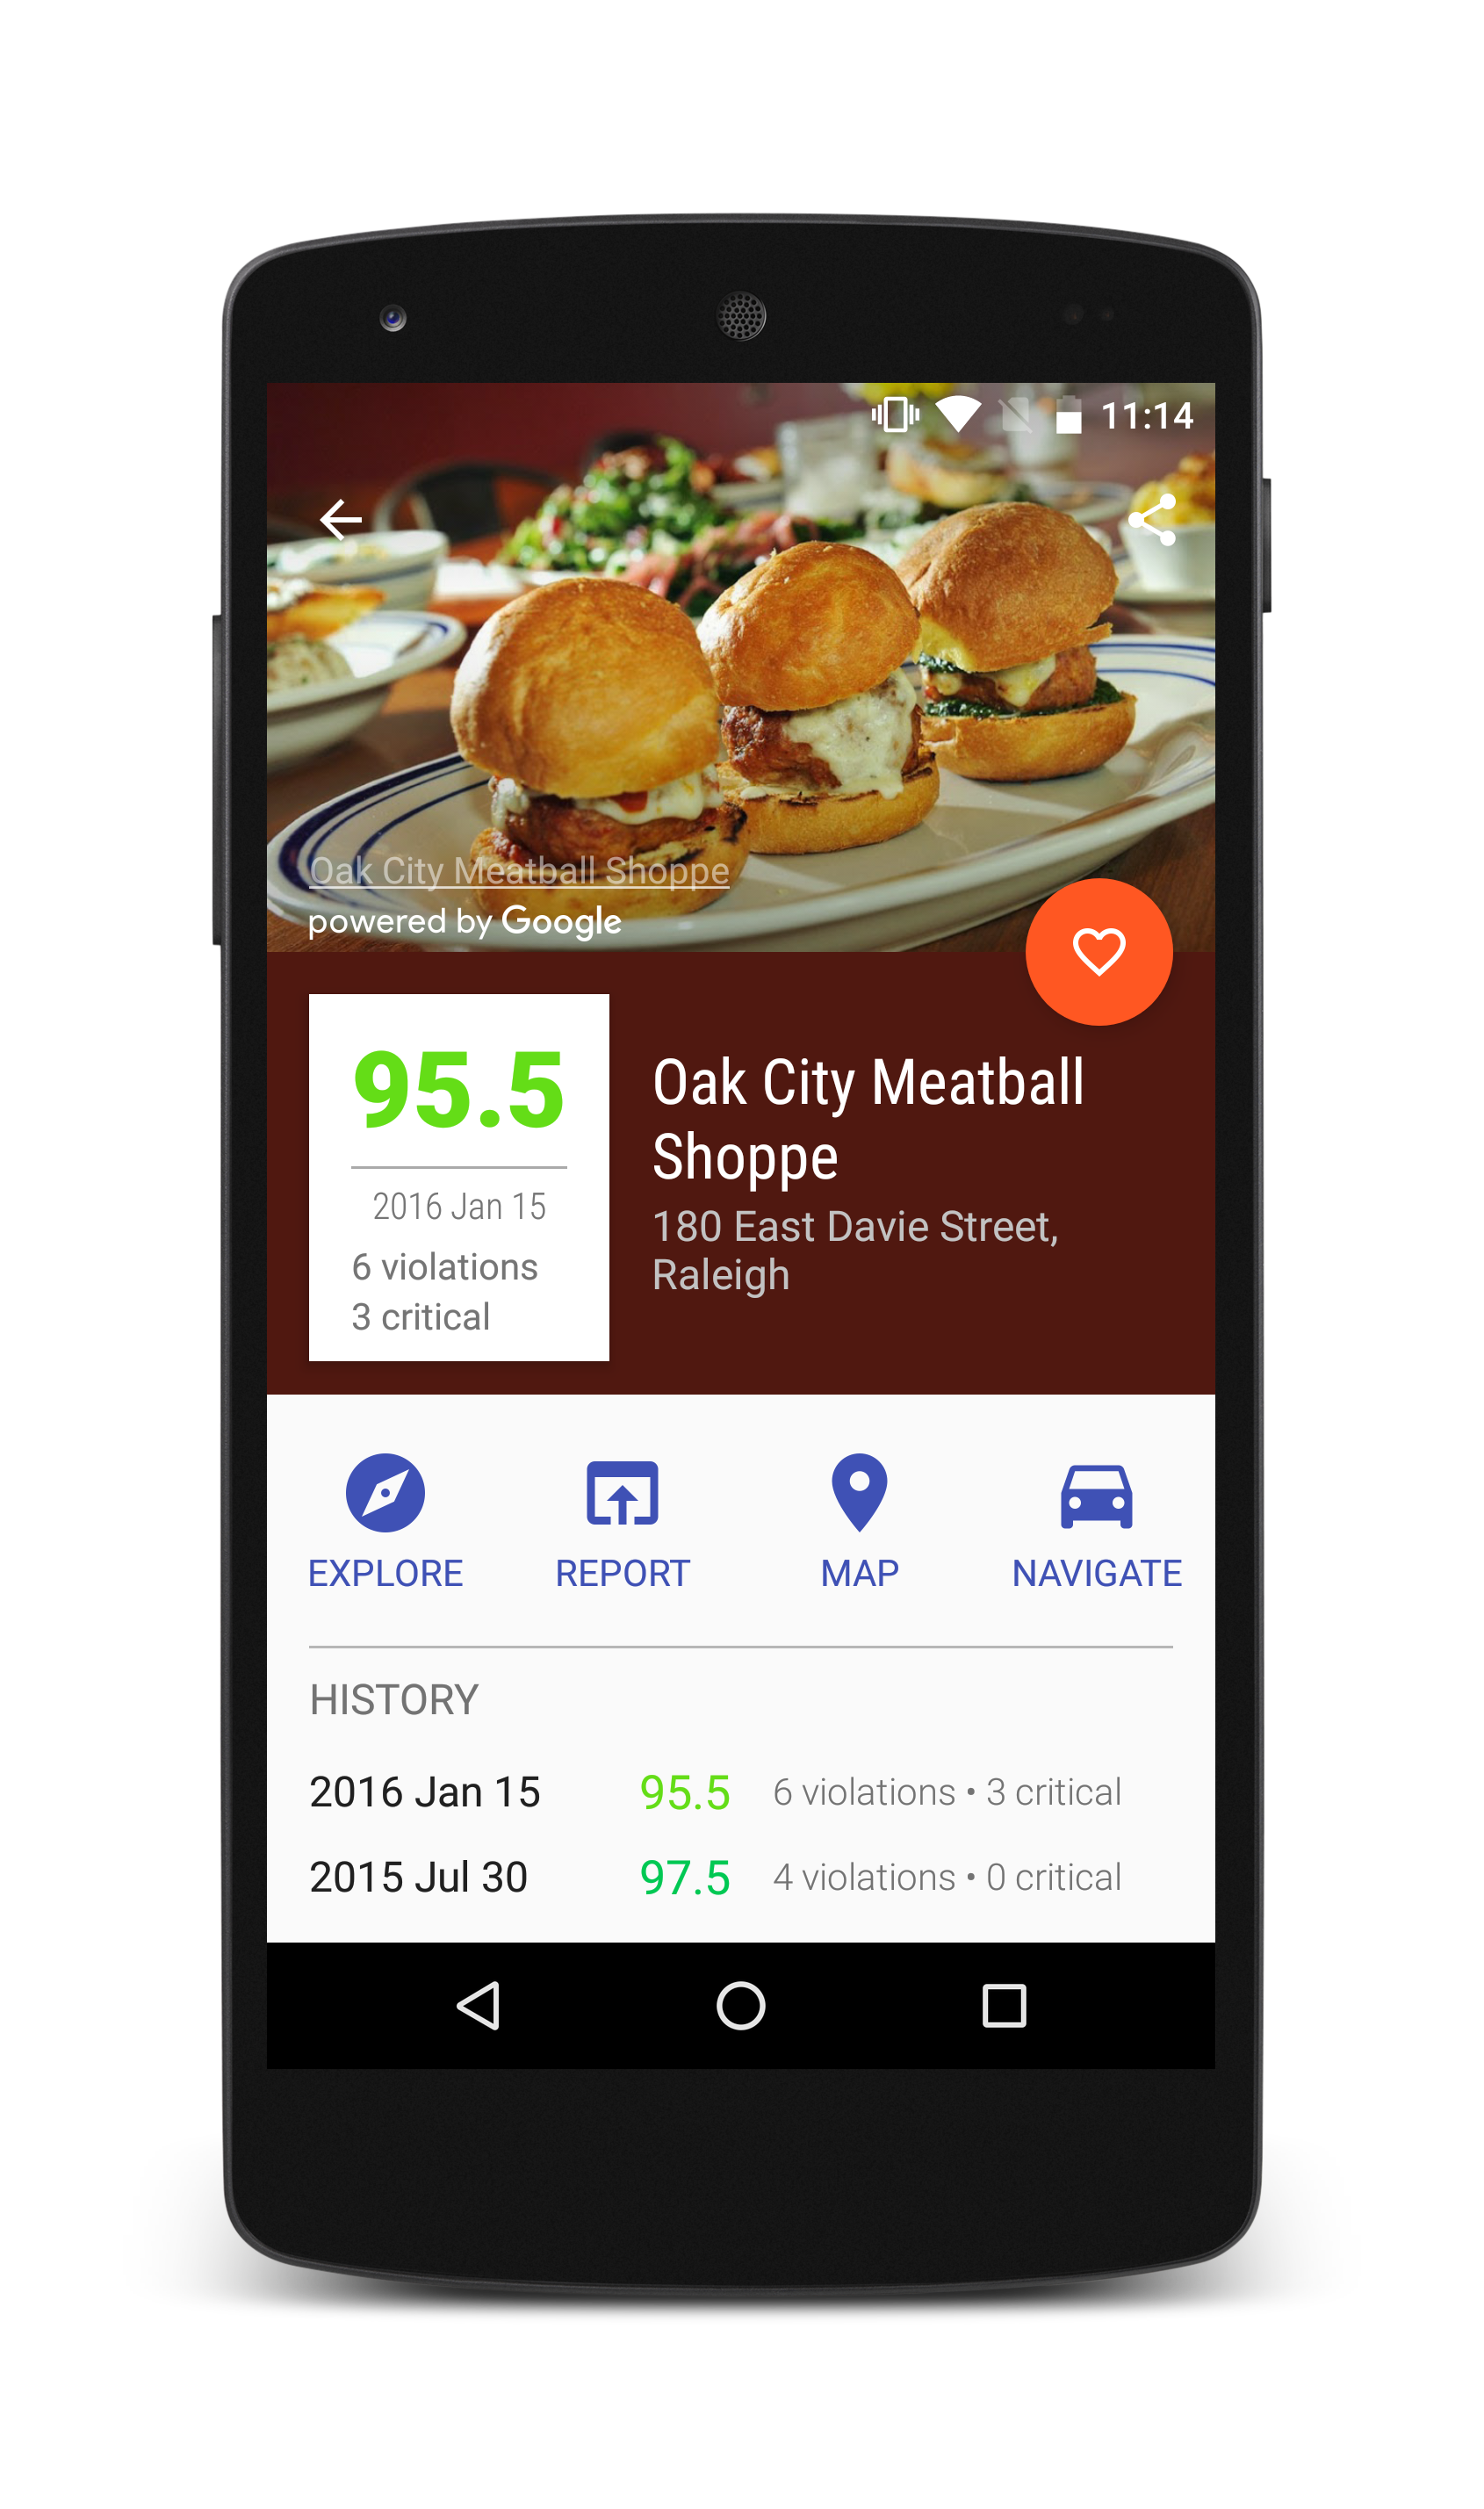
\includegraphics[width=0.45\textwidth]{html/ks_details_nexus5.png}
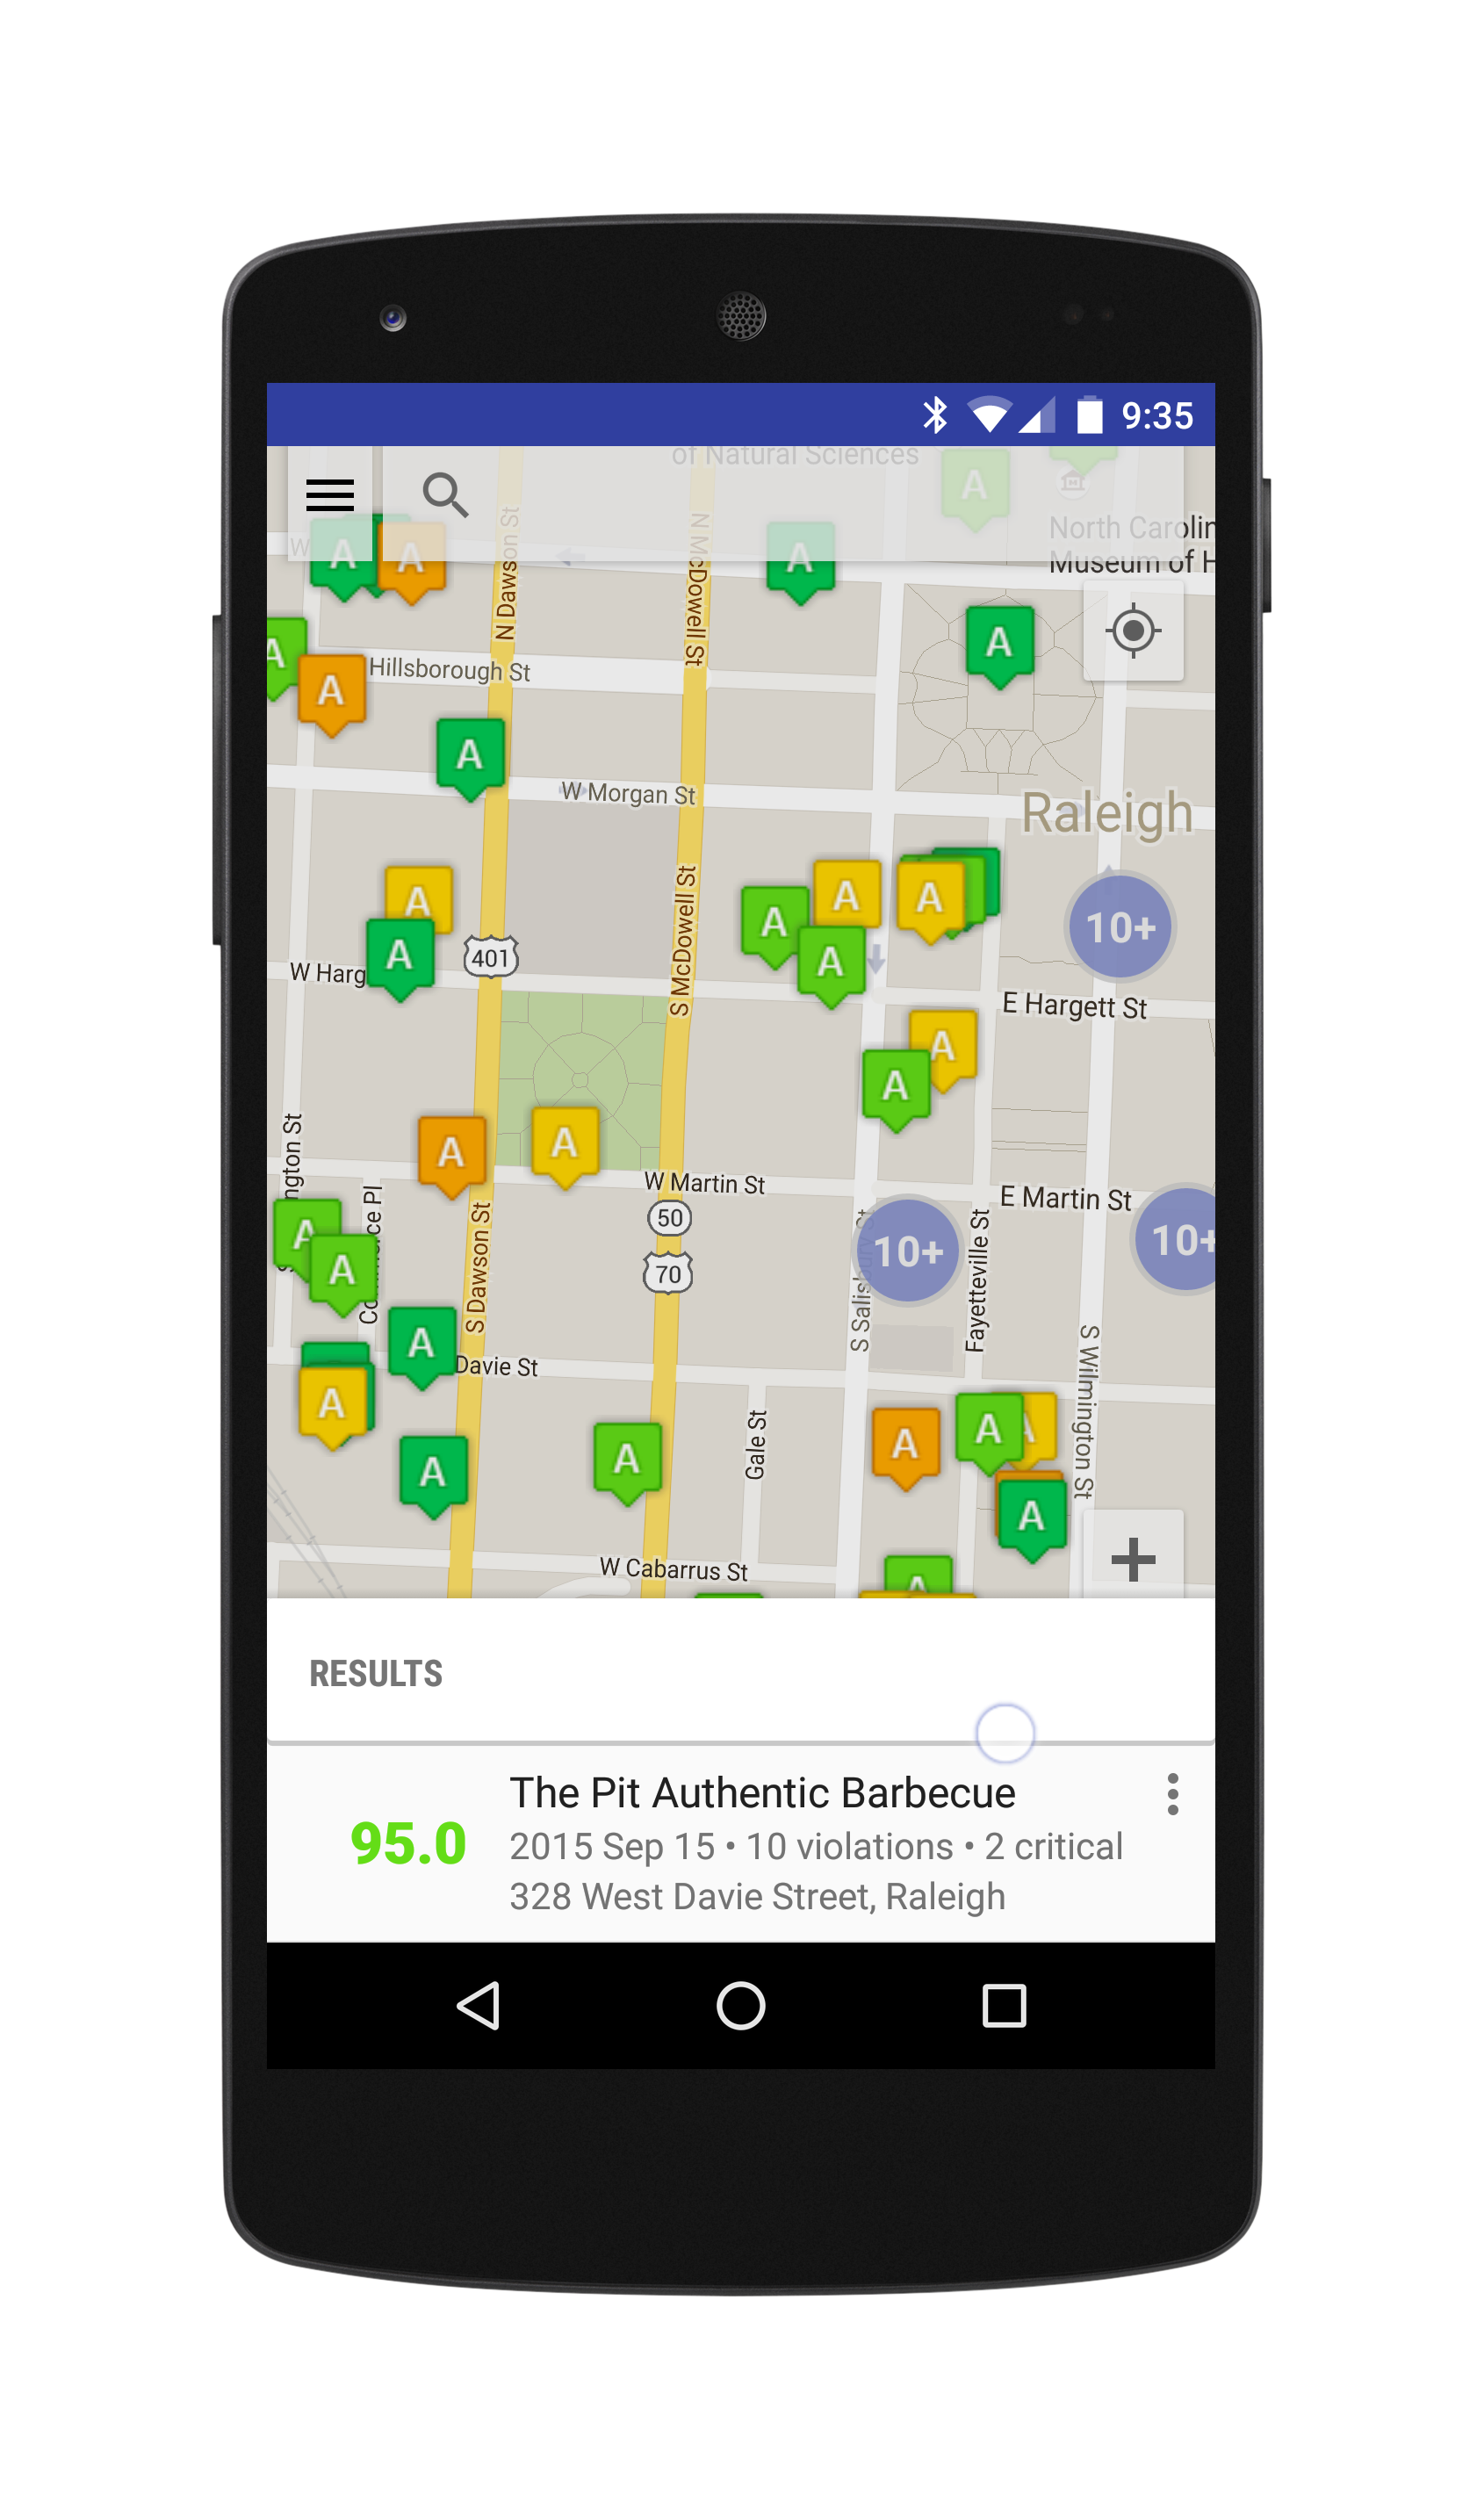
\includegraphics[width=0.45\textwidth]{html/ks_explore_nexus5.png}
\end{center}
%*endignore

Getting Kitchen Snitch:

The mobile client can be installed from the
\href{https://play.google.com/store/apps/details?id=com.honu.ksnitch}{Google
Play Store}. There is also a landing page
\mbox{\url{http://getks.honuapps.com/}}.

The Haskell server source code is available on darcshub.

\FurtherReading
\begin{compactitem}
 \item ks-rest \url{http://hub.darcs.net/dino/ks-rest}
 \item ks-download \url{http://hub.darcs.net/dino/ks-download}
 \item ks-library \url{http://hub.darcs.net/dino/ks-library}
\end{compactitem}

\end{hcarentry}
